\section{Resumen}

A raíz de la problemática expuesta en la sección anterior, el presente trabajo de memoria presenta un \emph{framework} de integración bidireccional entre un simulador de redes de comunicaciones inalámbricas -- OMNeT++ -- con un simulador de redes de transporte -- Quadstone Paramics -- como una herramienta de apoyo para el estudio de las problemáticas previamente señaladas y la evaluación de nuevos modelos y soluciones para transporte inteligente.

La elección de éstos simuladores en particular tiene razones bien fundadas. En particular, OMNeT++ fue escogido principalmente por particularidades que se verán más adelante, relacionadas con la elección de solución al problema planteado. Por otro lado, Paramics es el simulador de transporte de preferencia del Departamento de Transportes de la Universidad de Chile, parte interesada en el presente proyecto de memoria dadas las aplicaciones que puede tener para la investigación que se realiza en el Departamento. La extensión de Paramics para su funcionamiento en un sistema de simulación integrado bidireccional permitiría a su vez la extensión de modelos ya existentes que maneja dicha área de investigación, para sus estudios en contextos de Sistemas de Transporte Inteligente.

El \emph{framework} desarrollado para la memoria se implementó en base a una adaptación de un trabajo previamente realizado por Sommer \emph{et al.} \autocite{sommer_german_dressler, sommer_dressler2} para la integración de OMNeT++ con SUMO, otro simulador de redes de transporte. Este trabajo previo, un \emph{framework} denominado VEINS -- por sus siglas en inglés, \emph{Vehicles In Network Simulation} -- utiliza una novedosa arquitectura en la que ambos simuladores se comunican a través de un \emph{socket}, en una configuración cliente-servidor. La implementación presentada en este trabajo de memoria, denominada PVEINS\footnote{PVEINS -- \textbf{P}aramics \textbf{VEINS}}, pretende reemplazar, de manera absolutamente transparente para OMNeT++, a SUMO en dicha arquitectura, para así poder aprovechar todo el trabajo en modelos de comunicación ya existentes para esta configuración.

\begin{figure}[tpb]
    \centering
    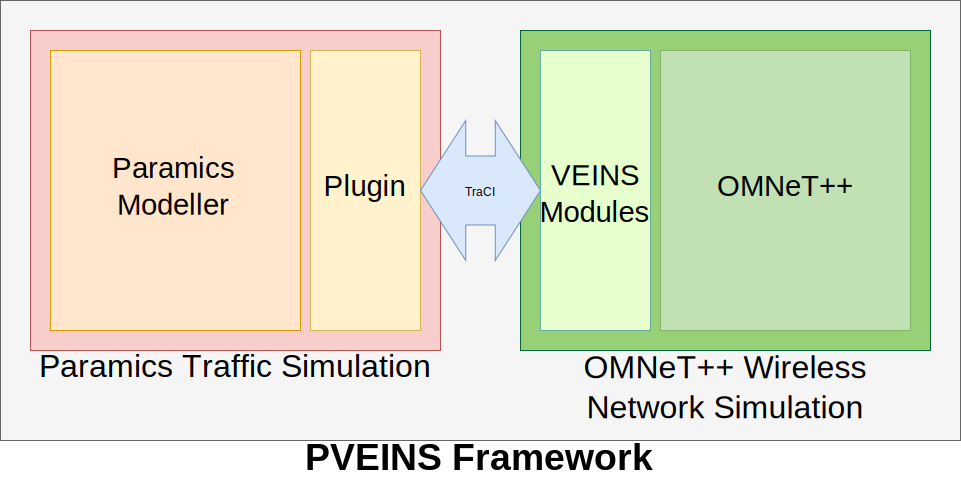
\includegraphics[width=\linewidth]{figuras/PVEINSArch.png}
    \caption{Integración bidireccional de Paramics con OMNeT++.}
    \label{fig:pveins_genarch:resumen}
\end{figure}

El trabajo consistió principalmente en el desarrollo de un \emph{plugin} de extensión de Paramics, el cual se encarga de recibir e interpretar comandos desde el simulador de redes, realizando las operaciones necesarias en el modelo de Paramics. Este se desarrolló en C++, en su estándar 2011, utilizando la API del software (ver apéndice \ref{anex:paramics_api}).

Este \emph{plugin} permite la integración de Paramics con el entorno de simulación de OMNeT++, posibilitando la simulación de Sistemas Inteligentes de Transporte -- el \emph{framework} permite al simulador de redes construir una red inalámbrica equivalente a la red de transporte simulada, donde cada vehículo en Paramics se asocia a un nodo dotado de capacidades de comunicación inalámbrica en OMNeT++. El estado de ambas simulaciones evoluciona de manera sincronizada, y los nodos de OMNeT++ están dotados de lógica y pueden modificar el comportamiento de sus respectivos vehículos. De esta manera, es posible analizar tanto el impacto de la movilidad de los vehículos sobre el canal de comunicaciones, como el impacto de la transmisión de información en el modelo de transporte.

Este nuevo \emph{framework} PVEINS se validó luego mediante una serie de experimentos destinados a medir su rendimiento y su aptitud para uso en investigación y modelación de Sistemas Inteligentes de Transporte de una complejidad considerable. El Área de Transportes del Departamento de Ingeniería Civil de la Universidad de Chile proporcionó un escenario realista que modela un sector de la ciudad de Santiago en hora punta, el cual se utilizó para la validación del \emph{software}. Este escenario es de alta complejidad, elaborado por Zúñiga \autocite{zuniga} en 2010 para su memoria de título, y presenta un promedio de aprox. 1400 vehículos presentes en la red en cada instante de la simulación. 

Los resultados de los análisis realizados sobre el \emph{framework} en el contexto de un escenario tan complejo como el proporcionado fueron altamente positivos. El software es eficiente, y permite modelar de manera precisa y realista el comportamiento de los Sistemas Inteligentes de Transporte.

Sin embargo, este trabajo de todas maneras identifica factores y detalles perfeccionables en la implementación del sistema, los cuales se presentan al final de este documento como sugerencias para trabajo futuro. 

Finalmente, el producto de este trabajo de memoria se encuentra disponible en su totalidad en el repositorio \emph{git} personal del autor \autocite{pveins_github}, bajo una licencia \emph{BSD 3-Clause} \autocite{bsd3clause}. Ahí se podrá encontrar tanto el código fuente del \emph{framework} como del escenario de validación avanzado y los resultados de las pruebas realizadas.